\documentclass[10pt,a4paper]{article}
\usepackage[a4paper,margin=1.5cm,top=1.0cm,bottom=0.8cm]{geometry}
\usepackage[T1]{fontenc}
\usepackage[scaled=0.95]{helvet}
\renewcommand{\familydefault}{\sfdefault}
\usepackage{booktabs,tabularx,array,enumitem}
\usepackage{tikz}
\usetikzlibrary{positioning,arrows.meta}
\usepackage{pgfplots}
\pgfplotsset{compat=1.18}
\pagestyle{empty}
\setlength{\parindent}{0pt}
\setlength{\parskip}{2pt}
\newcommand{\sect}[2]{\vspace{3pt}{\bfseries\normalsize\fontsize{11}{13}\selectfont #1.\ #2}\par\vspace{1pt}}
\renewcommand{\arraystretch}{1.08}
\setlist{nosep,leftmargin=1.4em}

\begin{document}
\fontsize{9.4}{11.4}\selectfont
{\bfseries\fontsize{15}{18}\selectfont Product Recommendation from Transaction History: Project Report}\par
\vspace{1pt}
Date: November 2026 \quad\textbar\quad Status: complete

\sect{1}{Goal}
Build a model that reads a bank customer's transaction history and predicts which of five products they are likely to take up: travel card, personal loan, investments, insurance or cashback plus. The best-scoring product is the one we offer.

\sect{2}{What was done}
\begin{itemize}
\item Created a practice dataset of 20,000 customers and 4.25 million transactions, planned with HLD/LLD design.
\item Adapted an open AI language model, Qwen3-1.7B, to this task, training it twice on Kaggle's free GPUs (about 4 and 6.5 hours).
\item Tested it on 5,069 customers from later months than the training data, against four other models.
\end{itemize}

\sect{3}{Our approach}
Most banks summarise each customer into totals, such as ``spend in the last 90 days'', and score those. Totals lose the order of events: a pay rise followed by investing can look the same as late fees followed by a loan. Our model reads the individual transactions in order, combines them with the customer's profile, and learns from both at the same time. Figure~1 shows the steps.

\vspace{3pt}{\centering
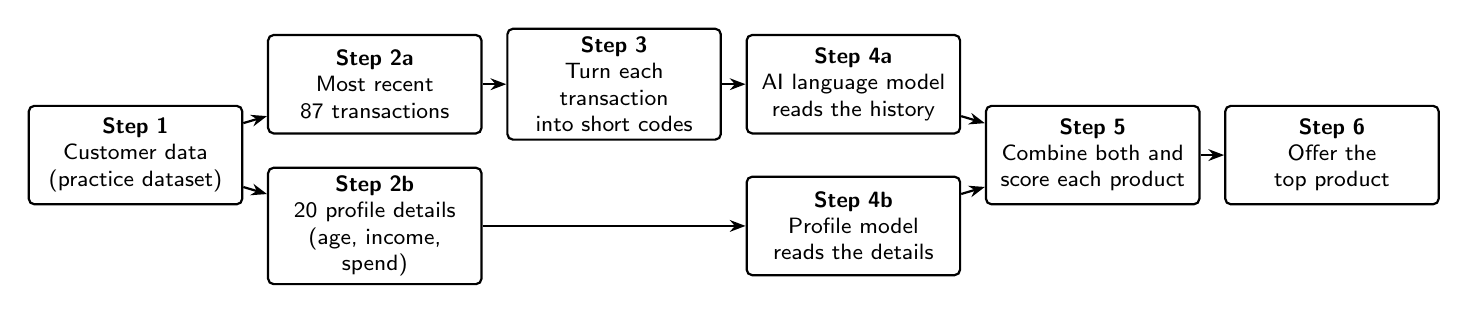
\begin{tikzpicture}[
  node distance=5mm and 3mm,
  b/.style={draw,thick,rounded corners=2pt,align=center,font=\footnotesize,minimum height=12.5mm,text width=25mm,inner sep=3pt},
  a/.style={-{Stealth[length=2mm]},thick}]
  \node[b] (gen) {\textbf{Step 1}\\Customer data\\(practice dataset)};
  \node[b,right=of gen,yshift=9mm] (tx) {\textbf{Step 2a}\\Most recent\\87 transactions};
  \node[b,right=of gen,yshift=-9mm] (tab) {\textbf{Step 2b}\\20 profile details\\(age, income,\\spend)};
  \node[b,right=of tx] (tok) {\textbf{Step 3}\\Turn each transaction\\into short codes};
  \node[b,right=of tok] (llm) {\textbf{Step 4a}\\AI language model\\reads the history};
  \node[b] (dcn) at (llm |- tab) {\textbf{Step 4b}\\Profile model\\reads the details};
  \node[b,right=of llm,yshift=-9mm] (fuse) {\textbf{Step 5}\\Combine both and\\score each product};
  \node[b,right=of fuse] (out) {\textbf{Step 6}\\Offer the\\top product};
  \draw[a] (gen) -- (tx);
  \draw[a] (gen) -- (tab);
  \draw[a] (tx) -- (tok);
  \draw[a] (tok) -- (llm);
  \draw[a] (tab) -- (dcn);
  \draw[a] (llm) -- (fuse);
  \draw[a] (dcn) -- (fuse);
  \draw[a] (fuse) -- (out);
\end{tikzpicture}\\[3pt]
{\small \textbf{Figure 1.} How a recommendation is made. In training, steps 4a, 4b and 5 learn together from whether the customer took the offer.}
\par}\vspace{2pt}

\sect{4}{Results}
Each model is scored on how well it ranks customers who took the product above those who did not: 0.5 means random guessing and 1.0 means perfect (this measure is called AUC). Our model scored 0.736, which is 3.8\% below the standard model (0.765).

\vspace{3pt}
\noindent\begin{minipage}[t]{0.6\linewidth}\centering
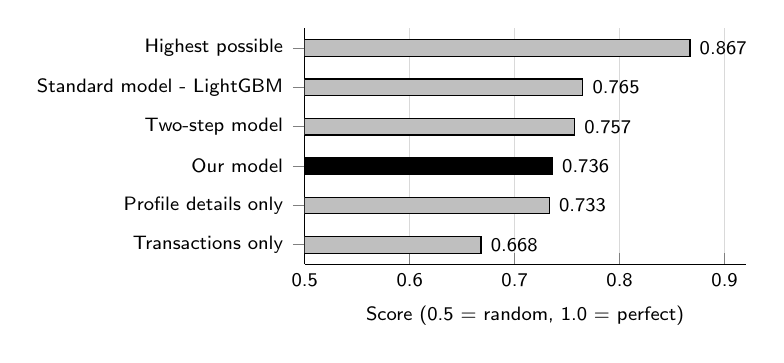
\begin{tikzpicture}
\begin{axis}[xbar, scale only axis, width=5.6cm, height=3.0cm, bar width=6pt, bar shift=0pt,
  xmin=0.5, xmax=0.92, xtick={0.5,0.6,0.7,0.8,0.9}, xticklabels={0.5,0.6,0.7,0.8,0.9},
  xlabel={Score (0.5 = random, 1.0 = perfect)},
  symbolic y coords={Highest possible,Standard model - LightGBM,Two-step model,Our model,Profile details only,Transactions only},
  ytick={Highest possible,Standard model - LightGBM,Two-step model,Our model,Profile details only,Transactions only}, y dir=reverse, enlarge y limits=0.1,
  point meta=explicit symbolic, nodes near coords, nodes near coords style={font=\scriptsize,anchor=west},
  every axis label/.style={font=\scriptsize}, tick label style={font=\scriptsize},
  axis x line*=bottom, axis y line*=left, xmajorgrids, grid style={black!15}]
\addplot[draw=black, fill=black!25] coordinates {(0.867,Highest possible)[0.867] (0.765,Standard model - LightGBM)[0.765] (0.757,Two-step model)[0.757] (0.733,Profile details only)[0.733] (0.668,Transactions only)[0.668]};
\addplot[draw=black, fill=black] coordinates {(0.736,Our model)[0.736]};
\end{axis}
\end{tikzpicture}\\[1pt]
{\small \textbf{Figure 2.} Test scores; our model is the black bar.}
\end{minipage}\hfill
\begin{minipage}[t]{0.37\linewidth}\centering
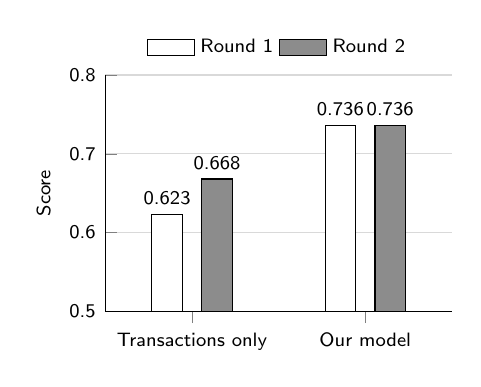
\begin{tikzpicture}
\begin{axis}[ybar=7pt, scale only axis, width=4.4cm, height=3.0cm, bar width=11pt,
  ymin=0.5, ymax=0.8, ytick={0.5,0.6,0.7,0.8}, yticklabels={0.5,0.6,0.7,0.8}, ylabel={Score},
  symbolic x coords={Transactions only,Our model}, xtick=data, enlarge x limits=0.5,
  point meta=explicit symbolic, nodes near coords, nodes near coords style={font=\scriptsize},
  area legend, legend style={font=\scriptsize,at={(0.5,1.03)},anchor=south,legend columns=2,draw=none},
  every axis label/.style={font=\scriptsize}, tick label style={font=\scriptsize},
  axis x line*=bottom, axis y line*=left, ymajorgrids, grid style={black!15}]
\addplot[draw=black, fill=white] coordinates {(Transactions only,0.623)[0.623] (Our model,0.736)[0.736]};
\addplot[draw=black, fill=black!45] coordinates {(Transactions only,0.668)[0.668] (Our model,0.736)[0.736]};
\legend{Round 1, Round 2}
\end{axis}
\end{tikzpicture}\\[1pt]
{\small \textbf{Figure 3.} Score in round 1 and round 2.}
\end{minipage}
\vspace{2pt}

\sect{5}{Problems found and how we solved them}
\vspace{3pt}{\centering
{\footnotesize
\begin{tabularx}{\linewidth}{@{}>{\raggedright\arraybackslash}p{0.25\linewidth}>{\raggedright\arraybackslash}X>{\raggedright\arraybackslash}p{0.24\linewidth}@{}}
\toprule
\textbf{Problem} & \textbf{What we did} & \textbf{Result} \\
\midrule
No real bank data available & Built a practice dataset that also records each customer's true chance of taking each product & We know the highest score possible \\
Transactions written as text are long, and the model reads amounts poorly & Replaced each transaction with short codes for amount range, date and shop name & About 12 codes per transaction \\
The model is too large to train fully on free GPUs & Trained only small add-on parts (about 1\% of the model), with memory-saving settings & Uses 7\,GB of a 16\,GB GPU \\
Risk of testing on data the model had already seen & Trained on months 1--8, tuned on month 9, tested on months 10--12 & A fair test on future customers \\
Round 1 saw only the last 37 transactions & Round 2 doubled how much history the model reads & Transactions-only score rose from 0.623 to 0.668 \\
Round 1 ranked the five products worse than chance & Round 2 gave each product its own score & Product ranking now better than chance \\
\bottomrule
\end{tabularx}}\\[3pt]
{\small \textbf{Table 1.} Problems found during the project and how each was handled.}
\par}\vspace{2pt}

\sect{6}{Conclusion}
The system works from start to finish on free hardware, and transaction history alone predicts take-up well above random. It does not yet beat the standard model, mainly because the training set is small (13,000 customers) and the model has not first learned spending patterns.

\sect{7}{Suggested steps to improve the results}
\begin{enumerate}
\item \textbf{Teach the model spending patterns first.} Train it to predict the next transaction, then to recommend.
\item \textbf{Use more customers and train longer.} Use 50,000+ training customers and three passes instead of one.
\item \textbf{Use a larger test set.} About 55,000 test customers are needed to measure small improvements reliably.
\item \textbf{Change one thing at a time,} so each training round shows clearly what helped.
\item \textbf{Get more computing time.} Round 2 already used 6.4 of Kaggle's 12 free hours; longer training needs a paid GPU.
\item \textbf{Test on real, anonymised bank data} when available, to confirm the results hold outside the practice dataset.
\end{enumerate}
\end{document}
